\chapter{Getting Started}
\section{Installing Everything}
First things first...we need to get everything together!
Blender is easy enough to install.  Head to \url{http://www.blender.org} with your favorite browser and download the appropriate version for your OS from the download section.  Blender doesn't care where you install it.  Just extract the archive and put it somewhere appropriate.  Alternatively, if you are running Linux you can use your distribution's package manager to install it.\begin{figure}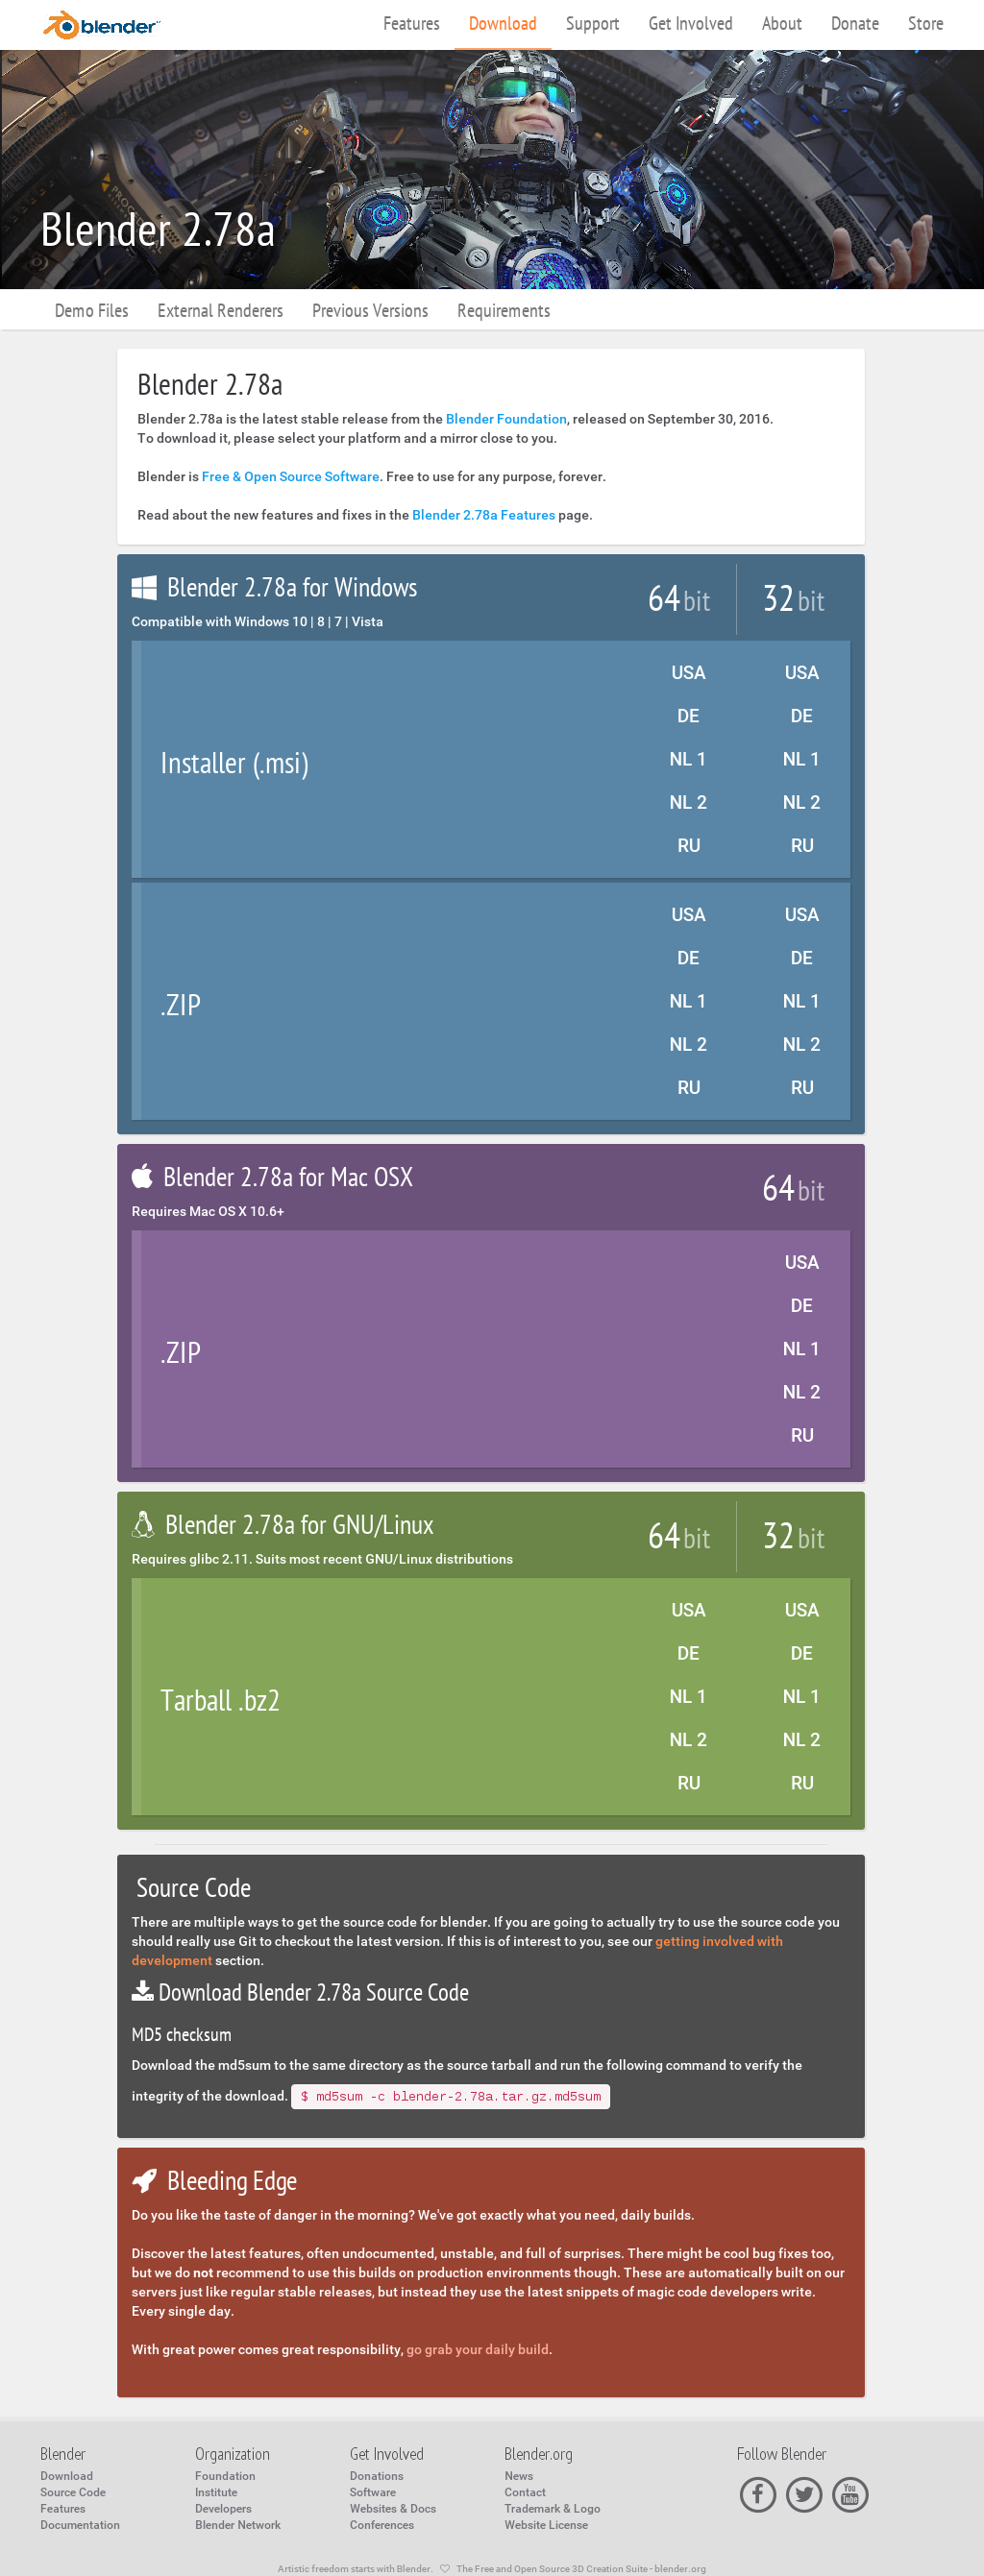
\includegraphics[height=2in]{blender001}	\caption{\url{http://www.blender.org/download}}\end{figure}
\todo{Fix flow of figure 1.1}
After installing Blender it is time to install PRMan.  To download PRMan you need to have a forum account at \url{http://renderman.pixar.com}.
\todo{Insert step-by-step for downloading PRMan}
\section{The Addon}
\todo{Discuss Addon Installation}
\section{Quick Renders}
\todo{Quick scene with default cube}
\section{Moving On}
\todo{Foreshadowing the rest of the book}

